\section*{Problem \#9}

\subsection*{Part 1}

$$
\begin{array}{l}
\dot{x}_{1}=x_{2} \\
\dot{x}_{2}=x_{1}-2 \tan ^{-1}\left(x_{1}+x_{2}\right)
\end{array}
$$

\noindent The behavior of this phase portrait is a bit unusual. While at first glance, it looke like a stable node, at the edges of the plot, we can see that there are diverging vector which might indictate that this system is more complicated than one might think at first glance.


\begin{figure}[h]
  \centering
  % 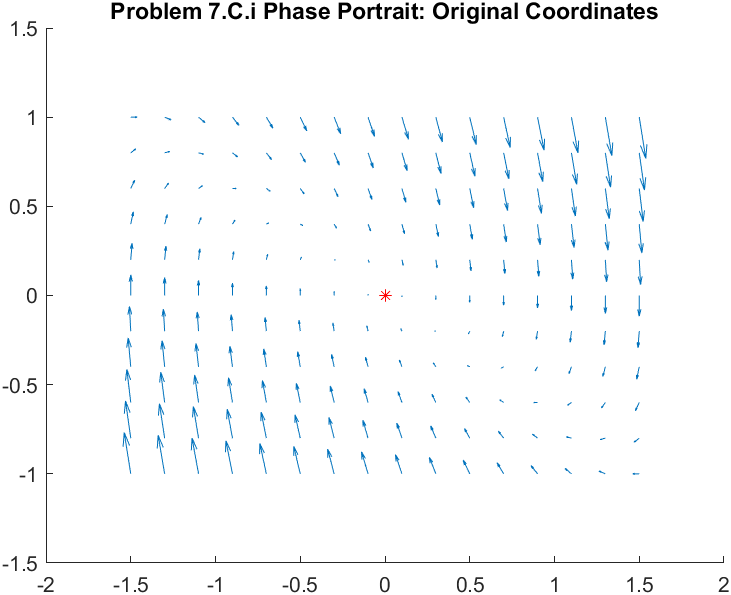
\includegraphics[width=\linewidth]{/prob7_img/7_C_i_Original}
  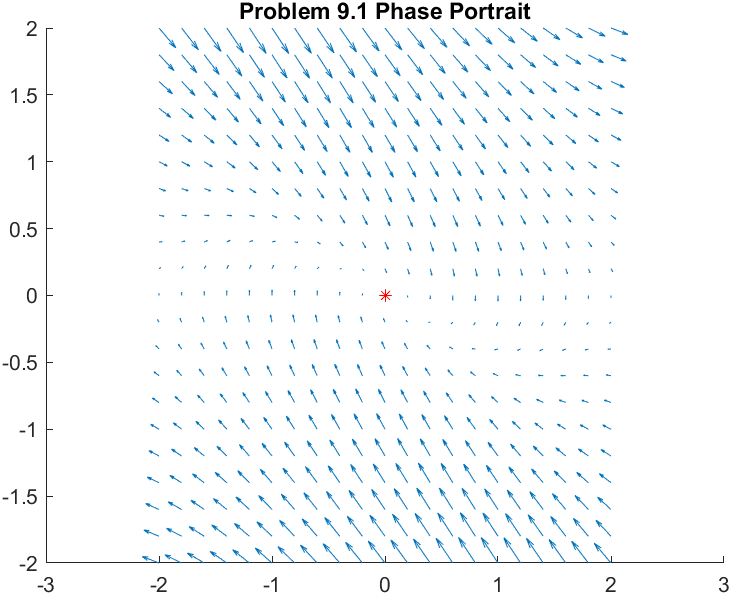
\includegraphics[width=\textwidth,height=.45\textheight,keepaspectratio]{/prob9_img/portrait_9_1}
\end{figure}

\subsection*{Part 2}

$$
\begin{array}{l}
\dot{x}_{1}=x_{2} \\
\dot{x}_{2}=-x_{1}+x_{2}\left(1-3 x_{1}^{2}-2 x_{2}^{2}\right)
\end{array}
$$

\noindent The behavior of this phase portrait is unsual in the fact that the vector field is approaching the $y = 0$ vertically from both the positive and negative directions. This might indictate that the system as a continuum, equilibrium along this line. The other interesting behavior of this system is that it the magnitude of the vector field is more pronouced at the extremes of the plot and quickly dies down in the neighborhood around the origin.

\begin{figure}[h]
  \centering
  % 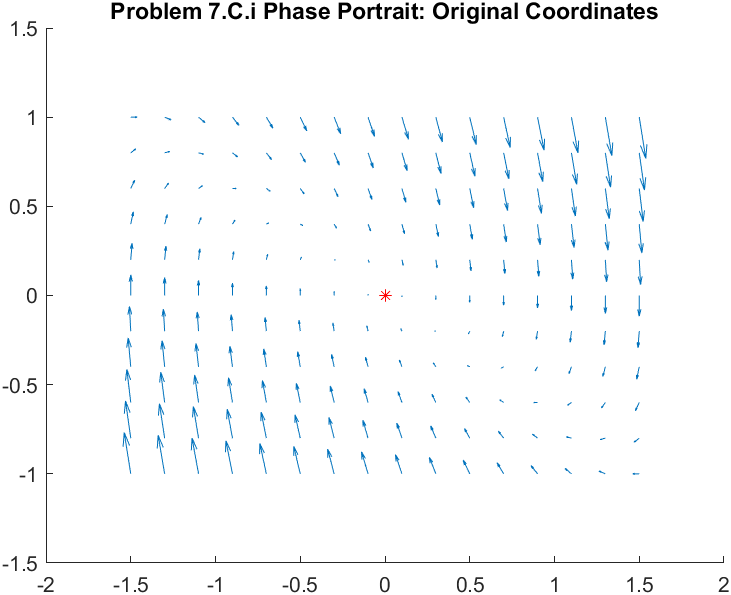
\includegraphics[width=\linewidth]{/prob7_img/7_C_i_Original}
  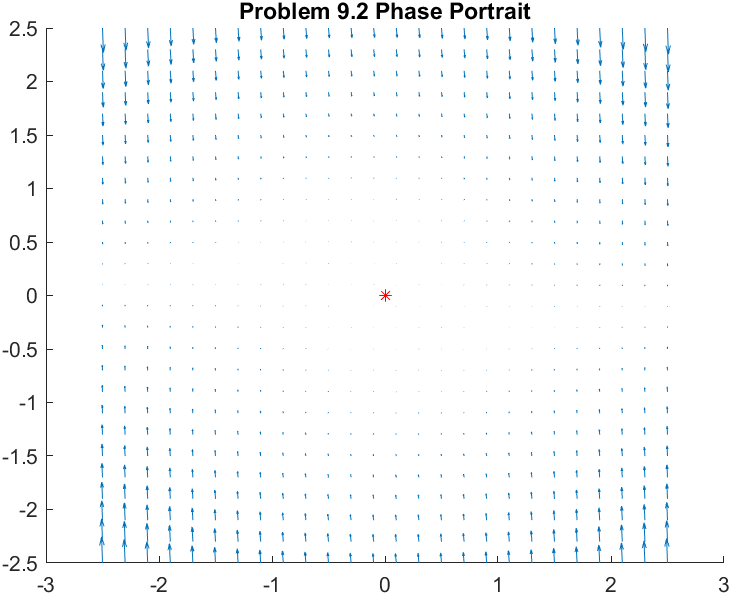
\includegraphics[width=\textwidth,height=.45\textheight,keepaspectratio]{/prob9_img/portrait_9_2}
\end{figure}


\subsection*{Part 3}

$$
\begin{array}{l}
\dot{x}_{1}=x_{1}-x_{1} x_{2} \\
\dot{x}_{2}=2 x_{1}^{2}-x_{2}
\end{array}
$$

\noindent This phase portrait apears to show that the system is strongly unstable about the origin (and the entire domain of the plot), as the vector field has a large magnitude throughout the plot. None of which converge to the origin. However, the most interesting feature of this plot is how regular the features are and how the system propigates to the left in almost perfectly horizontal lines. This means that from any initial condition starting inside the domain of the plane, the phase prortrait doesn't appear to converge, however it merely forces the system to transit to the left. While I cannot say for sure, in theory I could see this being the property of a vertical continuum equilibrium point at some point beyond the scope of the plot. However it is also possible that the system is actually well defined, but requires a must larger domain so that to see the pattern.

\begin{figure}[hb!]
  \centering

  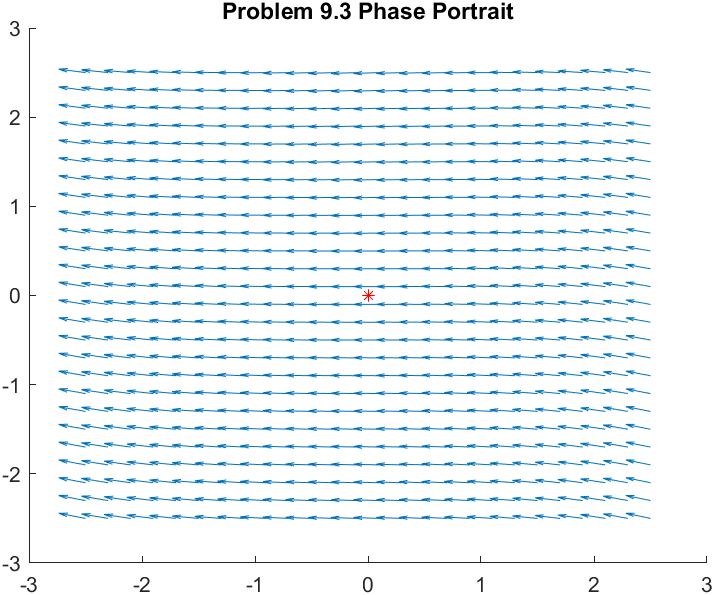
\includegraphics[width=\textwidth,height=.45\textheight,keepaspectratio]{/prob9_img/portrait_9_3}
\end{figure}


\subsection*{Part 4}

$$
\begin{array}{l}
\dot{x}_{1}=x_{1}+x_{2}-x_{1}\left(\left|x_{1}\right|+\left|x_{2}\right|\right) \\
\dot{x}_{2}=-2 x_{1}+x_{2}-x_{2}\left(\left|x_{1}\right|+\left|x_{2}\right|\right)
\end{array}
$$

\noindent Similar to the second phase protrait, we see what appears to be a continuous horizontal line of equilibrium at $y=0$. The vector fields approach that line nearly perfectly vertically from both the top and bottom directions. While this plot is very much like the other plot, the vector field about the line $x = 0$, is must more pronounced.

\begin{figure}[h]
  \centering
  % 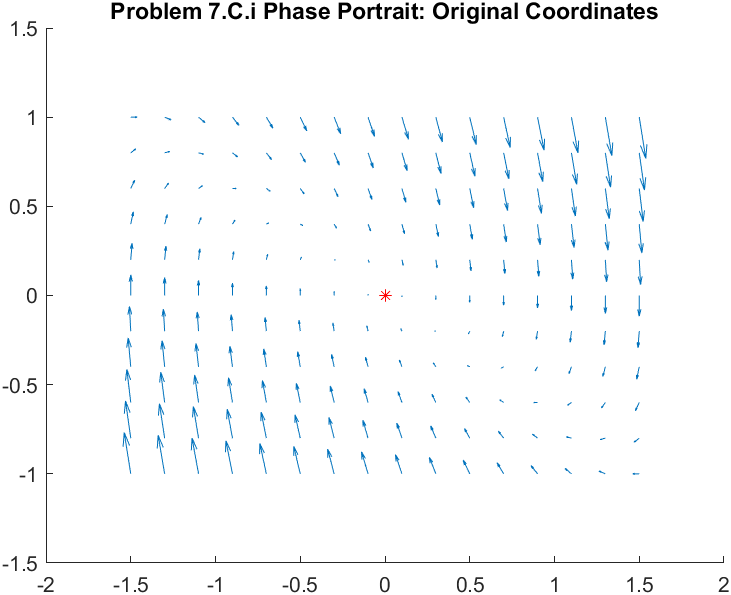
\includegraphics[width=\linewidth]{/prob7_img/7_C_i_Original}
  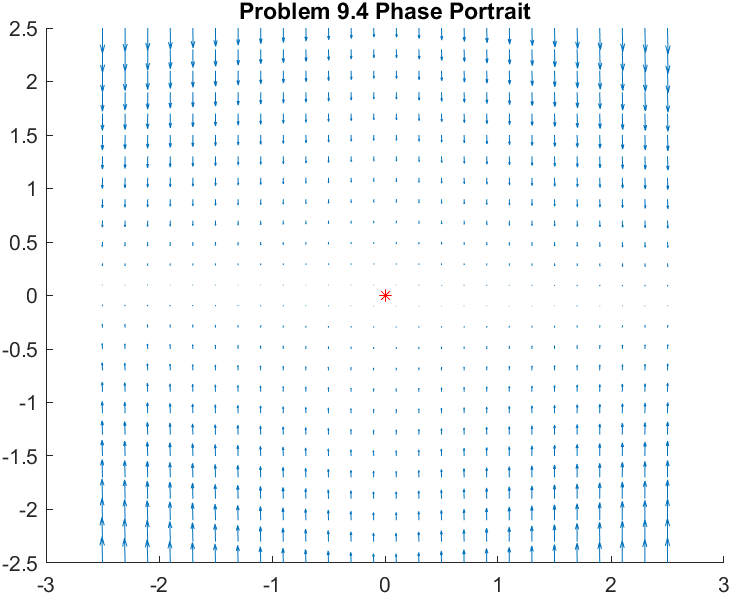
\includegraphics[width=\textwidth,height=.45\textheight,keepaspectratio]{/prob9_img/portrait_9_4}
\end{figure}
